%
% include the class file for USI-INF Technical Reports
%
\documentclass{usiinftr}
\usepackage{float}
\usepackage{amsmath}
\usepackage{slashbox}
\usepackage{subfigure}
\DeclareMathOperator*{\argmax}{argmax}



\begin{document}

\title{\bf Reproducibility challenge ATML SA 2021 \\ {\normalfont Generalization in Reinforcement Learning}}
\author{Erick Franciskus}{\dagger}
\author{Glejdis}{\ddagger}
\author{Constantin}{\ddagger}
\author{Jitin}{\ddagger}

\affiliation{\dagger}{Faculty of Informatics, Universit\`a della Svizzera italiana, Switzerland}
\affiliation{\ddagger}{Faculty of Engineering, Friedrich-Alexander Universit\"at Erlangen-N\"urnberg, Germany}



%
% by default, the current month and year are used as the publication date
% of your Technical Report; if you want to change this, then you can do it here, e.g.
%
%\date{February~\the\year}
%\date{August 2011}

\maketitle

\begin{abstract}
Sed ut perspiciatis unde omnis iste natus error sit voluptatem accusantium doloremque laudantium, totam rem aperiam, eaque ipsa quae ab illo inventore veritatis et quasi architecto beatae vitae dicta sunt explicabo. Nemo enim ipsam voluptatem quia voluptas sit aspernatur aut odit aut fugit, sed quia consequuntur magni dolores eos qui ratione voluptatem sequi nesciunt.
\vskip 1em
At vero eos et accusamus et iusto odio dignissimos ducimus qui blanditiis praesentium voluptatum deleniti atque corrupti quos dolores et quas molestias excepturi sint occaecati cupiditate non provident, similique sunt in culpa qui officia deserunt mollitia animi, id est laborum et dolorum fuga. Et harum quidem rerum facilis est et expedita distinctio. Nam libero tempore, cum soluta nobis est eligendi optio cumque nihil impedit quo minus id quod maxime placeat facere possimus, omnis voluptas assumenda est, omnis dolor repellendus.
\end{abstract}

\section{Introduction}
Reinforcement Learning is used in sequential decision making for training agents in complex tasks. The agent interacts with the environment which, based on the agent's action, provides the agent with some reward (positive or negative). The agent then uses this feedback to update its behaviour with the goal of being optimal. Although current RL agents have demonstrated great potential in a variety of activities, they face difficulties in transferring these agent's capabilities to new unseen tasks. This happens even when the tasks are semantically equivalent. In other words, existing reinforcement learning agents frequently learn policies that do not generalize well to environments different than those environments these agents are trained on. For example, the paper considered a jumping task, where we have an agent that needs to jump over an obstacle. The agent learns from image observations. In order for the agent to not collide with the obstacle, the agent needs to precisely time the jump at a particular distance from the obstacle. The various tasks consist of shifting the floor height or changing the obstacle position or both. If we train deep RL agents on some of these tasks where we vary the obstacle positions, they perform poorly at previously unseen locations (i.e. struggle to jump over the obstacle without hitting it).  The challenge tackled in the paper is to generalize to unseen positions of the obstacle and floor heights in the test tasks, while using only a finite number of training tasks or environments sampled from a distribution of tasks.
\\
A few proposed solutions to poor generalization, adapted from supervised learning, include regularization (such as l2-regularization, dropout or noise injection), Domain Randomization and Data Augmentation (such as RandConv, RAD, DrQ), which is being used more recently. The majority of these ideas centre around improving the learning process in order to fully harness decision-making process, and they rarely use properties of the sequential aspect such as similarity in actions across temporal observations. Instead, this paper takes advantage of the fact that when an agent operates in similar tasks, the agent shows at least short sequences of behaviours that are similar across these tasks.
In their approach, the authors train the agents to learn a representation where the states are close when the optimal behaviour of the agent in the current states and future states are similar. They use the notion of behavioural similarity as it has the property of good generalization to observations across different tasks. This behavioural similarity between states across various tasks is quantified using the Policy Similarity Metric (PSM), which is a state-similarity metric based on bisimulation. Moreover, to enhance generalization, the agent is trained to learn state embeddings. This is done using Contrastive Similarity Metric (CSM).

\section{Theory and Concepts}
\subsection{The $\pi$-bisimulation and Policy Similarity Metric} \label{sec: PSM}

\subsection{Policy Similarity Embeddings - PSEs}
Aiming for generalization of learned policies to related environments, the authors represent states in an embedding space, where closeness of states correlates with similar optimal policies. The embedding is built by self-supervised contrastive learning. Self-supervised learning refers to learning techniques that work without explicit annotations of the data. \cite{tian2021understanding} Instead, feedback signals are generated from the data itself. In this case this feedback comes from the policy similarity metric.   The contrastive instance of self-supervised learning works with positive pairs that are similar to each other, and negative or dissimilars pairs. \cite{Hadsell06dimensionalityreduction} The policy similarity metric d (introduced in Section \ref{sec: PSM}) is transformed to the similarity measure $\Gamma$ using the Gaussian kernel:
\begin{equation} \label{Gaussian Kernel}
\Gamma (x,y) = \exp ( -d(x,y)/ \beta) 
\end{equation}

For two state spaces $\chi' \subseteq \chi$ and $Y$ resulting from MDPs the positive pair ${( \tilde{x}_y , y) }$ is chosen as the one with highest similarity. Hence, $ \tilde{x}_y = \argmax_{x \in \chi'} \Gamma (x,y)$ , $y \in Y $.

All other states are grouped to negative pairs. Eventually, we aim to map unknown states into this embedding to infer successful policies. 
Therefore, a function is needed that maps states into the embedding. 
The contrastive loss to learn this mapping is inspired from SimCLR, which also uses self supervised learning and heavy data augmentation to create a representation space of images that can be used for classification. \cite{chen2020simple}. The contrastive loss is given by: 

\begin{equation}\label{contrastive loss}
l_{\theta} (\tilde{x}_y, y; \chi' ) = 
- \log \frac{\Gamma (\tilde{x_y}, y ) \exp(\lambda s_{\theta} (\tilde{x}_y, y))}
{\Gamma(\tilde{x}_y, y) \exp (\lambda s_{\theta}(\tilde{x}_y, y)) + \sum_{x'\in \chi' \setminus {\tilde{x}_y}} (1 - \Gamma (x',y)) \exp (\lambda s_{\theta} (x',y))}
\end{equation}
This mapping function $z_\phi$ is composed of an encoding $f_\phi$ leading to the latent representation of the state and a non-linear projection $h_\phi$, following SimCLR. The contrastive loss (Equation \ref{contrastive loss}) is applied to the projection to train the network. The inference of a suitable policy is done in the representation space as an affine function $\pi_\theta (\cdot \mid y) = W^T f_y + b$
with learnable parameters W and b. The training procedure is depicted in the Figure \ref{fig: Learning_Architecture}.

\begin{figure} 
\centering
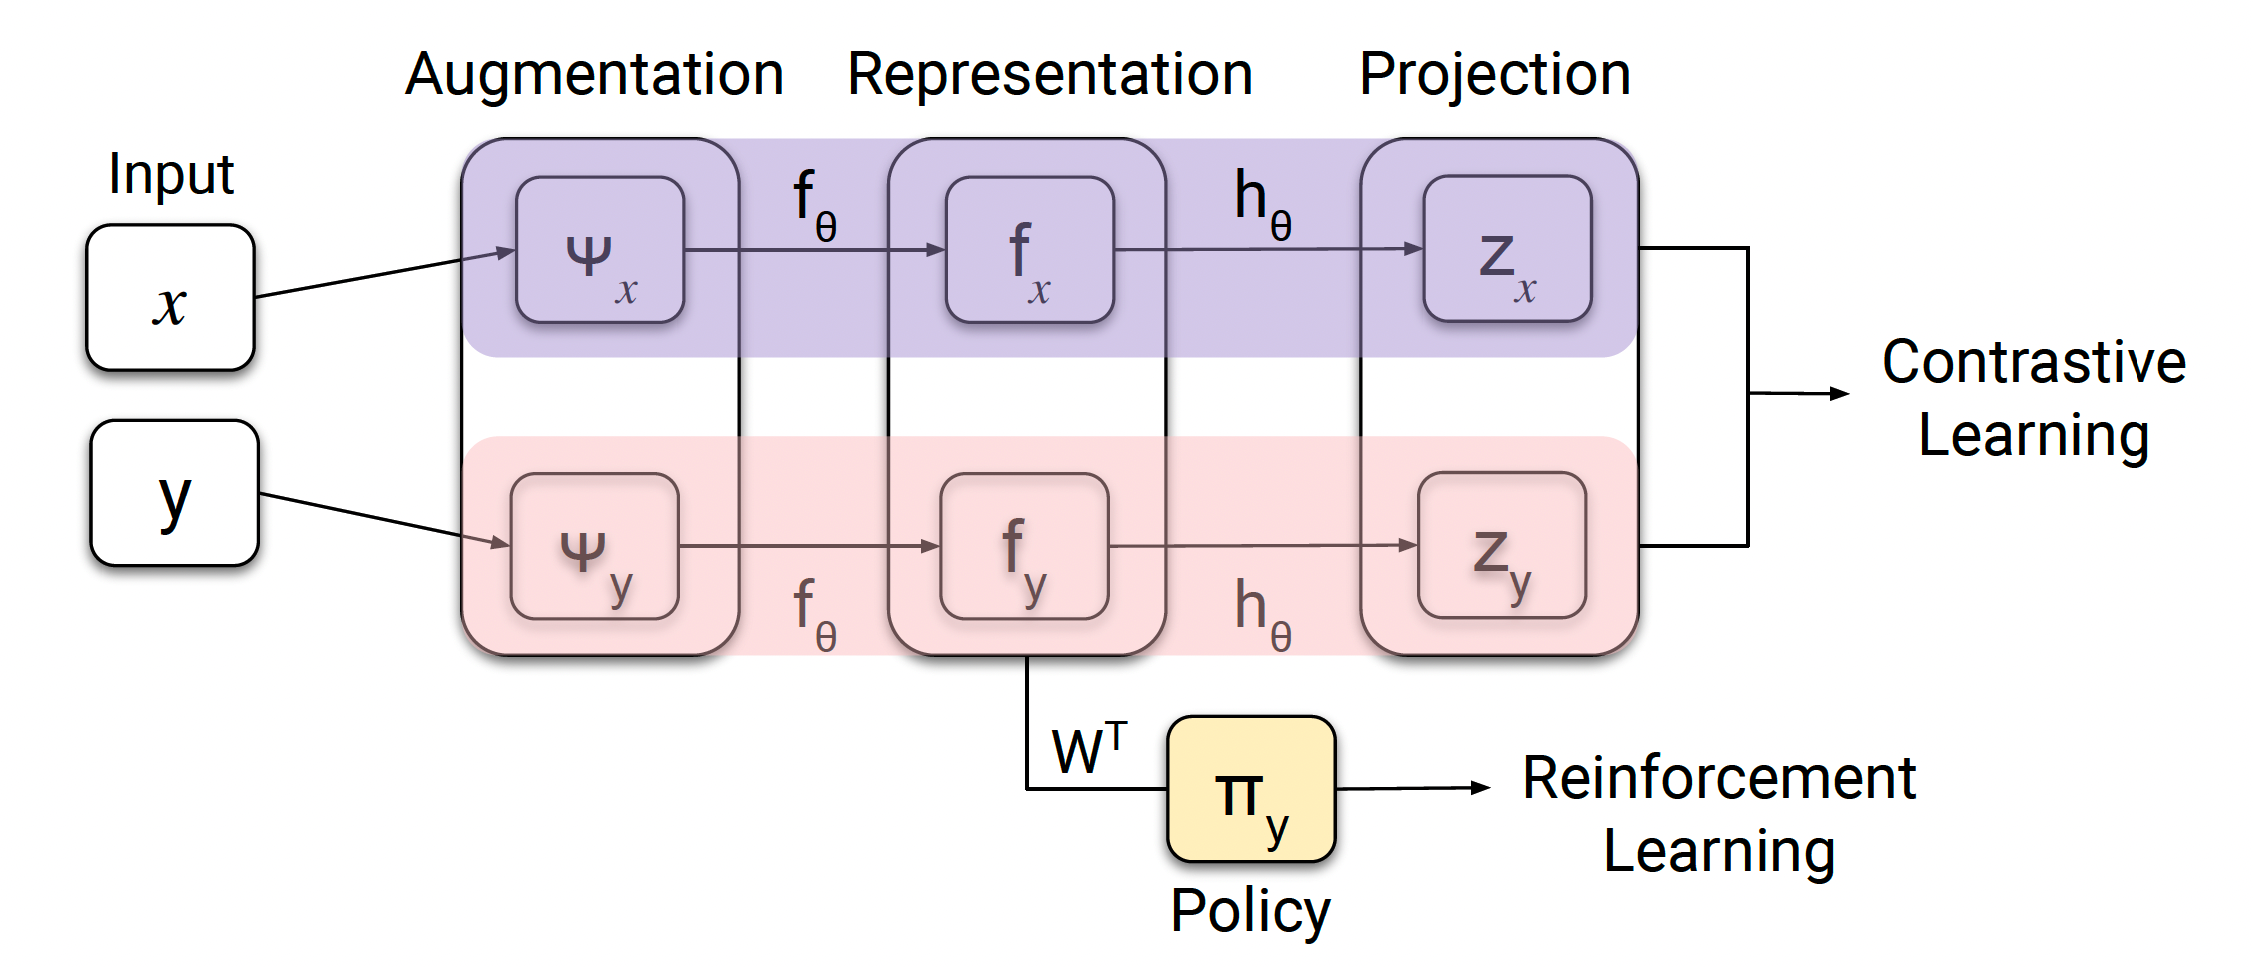
\includegraphics[width = 0.8\textwidth]{figures/Learning_architecture.png}
\caption{\label{fig: Learning_Architecture}An input pair (x,y) is first augmented and then mapped into the representation space $f$. The loss function defined in Equation \ref{contrastive loss} is applied to a non-linear projection $z$ of this representation space. \cite{agarwal2021contrastive} }
\end{figure}

The contrastive metric embeddings learnt with policy metrics are referred to as policy similarity metrics. They are learnt simultaneously during training, where an auxiliary objective derived from the contrastive loss is introduced.
The total contrastive loss for the MDPs $\mathcal{M}_\chi$ and $\mathcal{M}_y$ are derived from the optimal trajectories $\tau_\chi^* = \{x_t\}_{t = 1}^N$ and $\tau_y^* = \{y_t\}_{t = 1}^N$.
$x_t$ and $y_t$ are the single states in the optimal trajectories. $x_{t+1}$ is the result of applying the optimal policy $\pi^*$ to transition dynamics $P$ of the system : $x_{t+1} ~P_\chi^{\tau^*} (\cdot \mid x_t)$ and similar
$y_{t+1} ~ P_y^{\tau^*} (\cdot \mid y_t)$.
The authors set $\chi' = \tau_\chi^*$ (compare to Equation \ref{contrastive loss}) and then define the total contrastive loss as:

\begin{equation}
L_\theta (\mathcal{M}_\chi, \mathcal{M}_y) = \mathbb{E}_{y \sim  \tau_y^*} [l_\theta (\tilde{x}_y, y;\tau_\chi^*)] . 
\end{equation}

$\tilde{x}$ is chosen as the most similar state to the given state y: $\tilde{x} = \argmax_{x \in \tau_\chi ^ *} \Gamma (x,y) $ . Then the loss between the Markov processes $\mathcal{M}_\chi$ and $\mathcal{M}_y$ are hence the expected value for y from the optimal trajectory of the contrastive loss (Equation  \ref{contrastive loss}) of $\tilde{x}$ and $y$ w.r.t. to the optimal trajectory of $x$.  The loss becomes low, if we can conclude states $\tilde{x}$ that are close w.r.t. its optimal trajectory from the similarity, in the representation space, to y. 

\section{Experiments from the paper}
In this section we want to introduce the paper's main experiment: the jumping task from pixels. The authors also studied generalization on the dm control suite where agents have to ignore visual distraction. However, we want to focus our reproducibility study on the jumping task.
\subsection{Jumping Task from Pixels: A Case Study}
In the jumping task, we have an agent that, learning from the image observations on pixel level, needs to jump over an obstacle. The agent can either go right or jump. To avoid a collision the agent needs to time the jump precisely. The environment can be adapted by changing the floor height and the position of the obstacle. Two possible environments and their optimal trajectory are shown in Figure \ref{fig: optimal_trajectories}. Generalization is reached, when the agent becomes invariant to such changes.
There are 26 different positions of the obstacle and 11 different values of the floor height. To stress generalization, the problem is split into 18 training tasks and the remaining 268 tasks are evaluation tasks.
\begin{figure} 
\centering
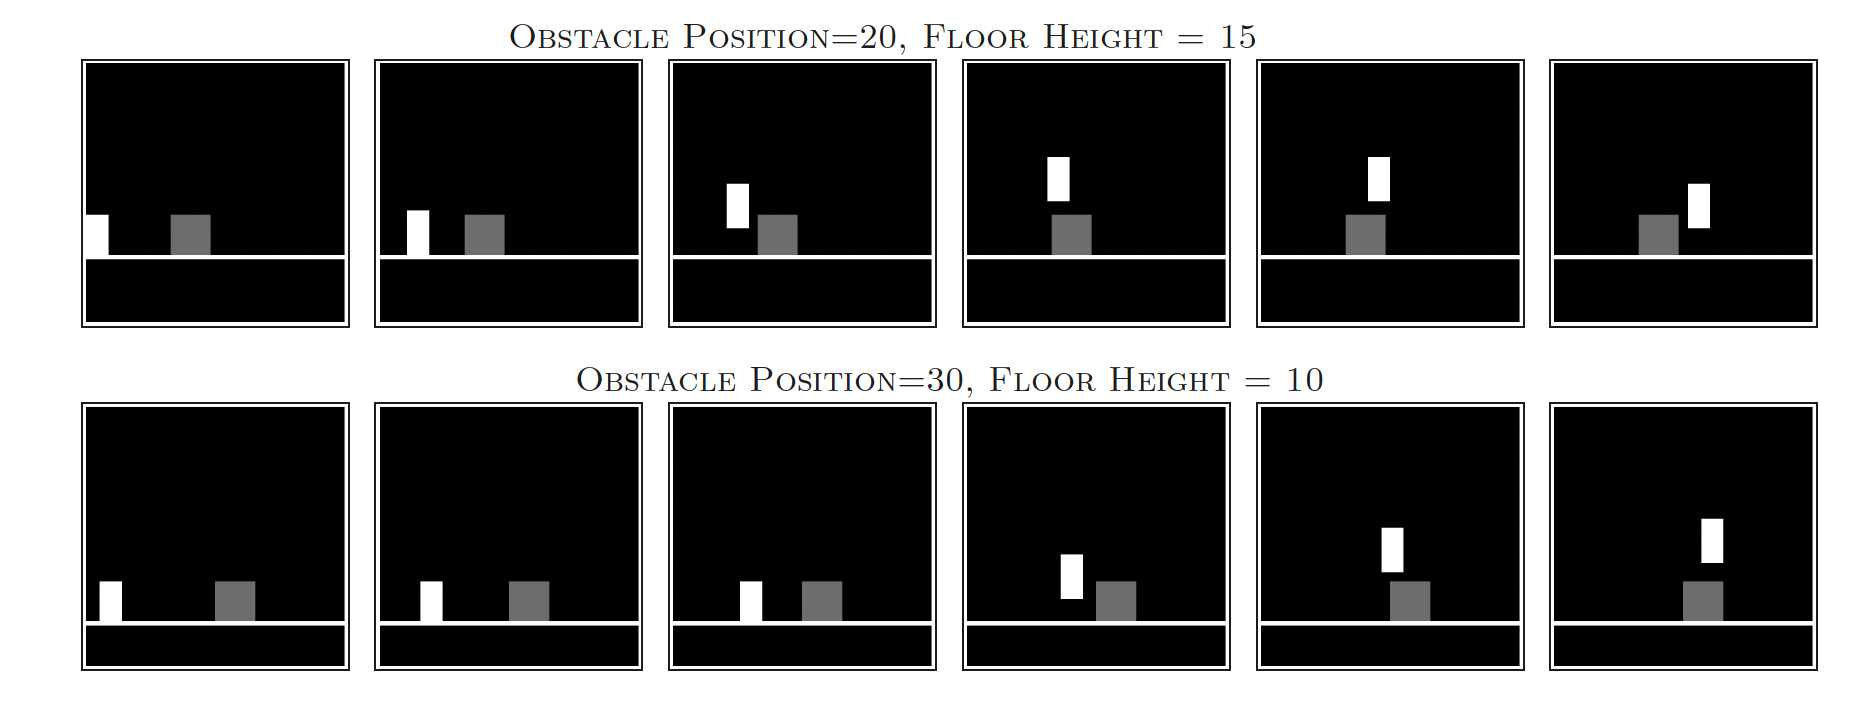
\includegraphics[width = 0.8\textwidth]{figures/optimal_trajectories.png}
\caption{\label{fig: optimal_trajectories}Optimal trajectories are shown for two different environments. The trajectory is a sequence of right actions interrupted by a single jump action. \cite{agarwal2021contrastive} }
\end{figure}


\subsection{Classification of the problem}
The states of the environment are discrete. This becomes apparent as we are able to classify all possible problems in a grid as combinations of obstacle position and floor height in Figure \ref{fig: grid_results}.
The actions of the agent are discrete as well: go right or jump.
The problem is deterministic because the optimal trajectory can be concluded with certainty.
In particular, by processing the fully observable input: all pixel values are available to the agent.
Furthermore, the problem is stationary because the optimal trajectory for a given task is time-invariant.
As the agent is the only active participant in the environment the problem can be considered a single agent task.
\\
So the task actually falls into the "easiest" category of tasks for reinforcement learning. However, the aim of the authors is to study and improve generalization in RL. And the notion of generalization is very clear in this task and also measurable. Therefore, we think the task is very well chosen to study and show the ability of PSEs to improve generalization in RL.
\subsection{Results from the paper}
In the paper, three different grid configurations, that represent different styles of generalization are used:
\begin{itemize}
\item The wide grid tests generalization via interpolation
\item The narrow grid tests out-of-distribution generalization via extrapolation
\item The random grid evaluates generalization like supervised learning where the training and test samples are drawn i.i.d. (independently and identically distributed) 
\end{itemize}
All configurations are evaluated using the same hyperparameters that were tuned on the "wide" grid to show the robustness of PSEs to hyperparameter tuning. The authors compare the PSE to other regularization methods. Also the effect of data augmentation using RandConv is studied. RandConv is a recently proposed data augmentation method to improve generalization in RL. It uses a randomized convolutional neural network to perturb input observations randomly. \cite{lee2020network}. The average performance across 100 runs is reported in Figure \ref{fig: tabular_results}. 

\begin{figure} 
\centering
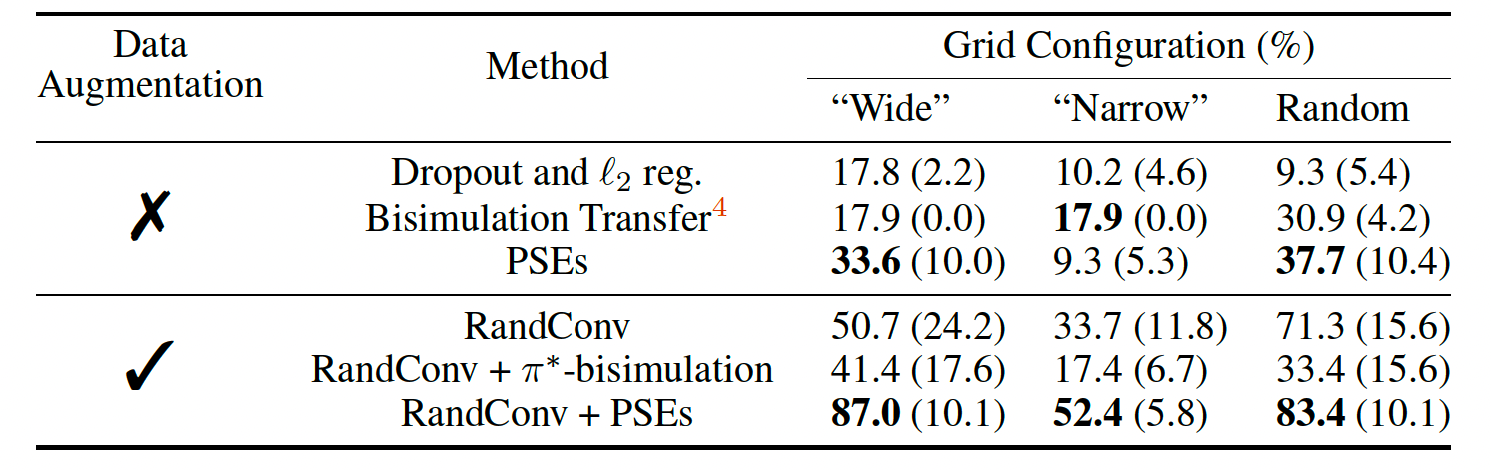
\includegraphics[width = 0.8\textwidth]{figures/tabular_results.png}
\caption{\label{fig: tabular_results}The table summarizes the main results of the authors, giving percentages of how many test tasks could be solved using different methods with or without data augmentation. The grid configurations are shown in Figure \ref{fig: grid_results}. It can be observed that PSEs outperform the compared methods in most configurations except for the narrow grid without data augmentation.
Also, PSEs profit substantially from data augmentation. \cite{agarwal2021contrastive}}
\end{figure}

PSEs outperform all other methods except for the case without data augmentation on the narrow grid. It is also apparent that PSEs work particularly well with data augmentation.
The different grid types as well as the performance of PSEs + data augmentation are shown in Figure \ref{fig: grid_results}.

\begin{figure} 
\centering
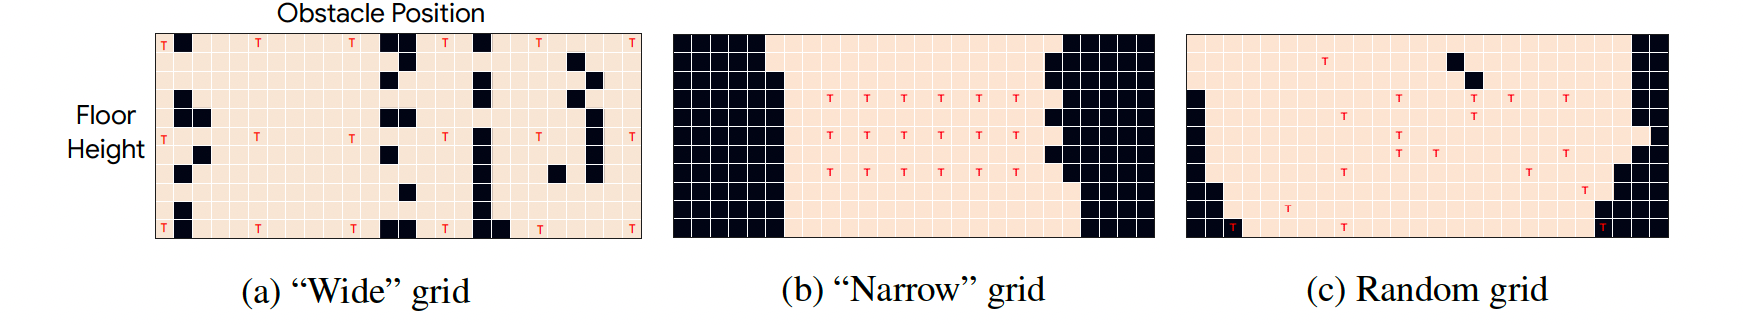
\includegraphics[width = 1\textwidth]{figures/grid_results.png}
\caption{\label{fig: grid_results}The red letter T shows which are the training tasks for the three grid configurations and the background colour of each tile shows the performance of PSEs accross the task configurations, which is reported as the median of 100 runs per configurations using data augmentation. Beige tiles correspond to tasks that could be solved and black tiles could not be solved. \cite{agarwal2021contrastive}}
\end{figure}

\bibliographystyle{plain}
\bibliography{citations}

\end{document}

